\section{Related Work}
\label{sec:StateOfTheArt}

Several virtual agents have been developed to study the impact of specific rapport strategies on the user perception of naturalness and social behaviour adequacy. The following sections describe the state-of-art in rapport and agents that are capable, at some extent, of managing rapport.

Section~\ref{sub:sec:ComputationalModelsOfRapport} describes current theoretical models for building rapport agents. Sections~\ref{sub:sec:rulebasedAgents}, \ref{sub:sec:datadrivenbasedAgents} describe virtual agents based on rules and \ac{ML} classifiers, respectively. Section~\ref{subsec:RestrictedPerceptionsWOZStudy} briefly describes current methodologies to learn social behaviours from \ac{WoZ} studies.

Lastly, Section~\ref{subsec:RelWorkDiscussion} discusses the current state-of-art and makes a brief comparison between the most important systems and their relevance and contribution to the proposed solution.

\subsection{Theoretical Models of Rapport for Agents}
\label{sub:sec:ComputationalModelsOfRapport}

Rapport is a mostly unconscious phenomenon~\cite{Zwiers2011} that occurs during interactions marked by strong perceptions of coordination, positivity and mutual attention.

The most important concepts for managing rapport are: planning social behaviours (Figure~\ref{table:BuildingRapportPlan}), learning social behaviours and flexible mechanisms to regulate current actions. Rapport models involve several complex cognitive mechanisms. Therefore it is beneficial to discretise it into smaller sets capable of, for example, enhancing positivity (friendliness) using self-disclosure or enhancing coordination and attentiveness through backchannel and turn-taking strategies~\cite{Sacks1974, Kahn2008, Welbergen2012}. The latter strategies are allied with good listeners as they must able to understand how to provide well-timed adequate feedback (backchannel) and identify appropriate moments to become the speaker (turn taking) and incite further dialogue~\cite{Sacks1974, Poppe2010}.

Zhao, Papangelis, and Cassell, propose a theoretical model to manage long-term rapport~\cite{Zhao2014, Papangelis2014} that is very relevant for current implementations of long-term social companionship agents~\cite{Lisetti2013, Bickmore2005, Kang2005}. Similarly to what was described previously in Section~\ref{subsec:Rapport}, the proposed model treats rapport as an interactional goal that is satisfied through strategies and actions according to the current state of the interaction and the user model (See Table~\ref{table:TCArchitectureDyadicRapportManagement:State}).

The strategies and the selected actions, despite initially representing the general sociocultural norms, must adapt to the interpersonal norms of the relationship and the context~\cite{Zhao2014}. As the relationship evolves, the dyadic state and the internal models should be updated in order to store the most accurate description of the interaction and return better behavioural responses that satisfy the dyad behavioural expectations~\cite{Papangelis2014}.

\vspace{-3mm}
\begin{table}[]
    \centering
    \begin{tabular}{@{}ll@{}}
        \toprule
        
        \multirow{1}{*}{\textbf{Dyadic State}} & Rapport State; Behavioural model; Friendship Status; History \\ \midrule
        \multirow{2}{*}{\textbf{User Model}} & User goals; Shared knowledge; Task model; \\  
        & Conversational Agent putative dyadic state \\ \bottomrule        

    \end{tabular}
    \caption{Relevant data structures for rapport models. Adapted from~\cite{Zhao2014}.}
    \label{table:TCArchitectureDyadicRapportManagement:State}
\end{table}
\vspace{-7mm}

Another important aspect for managing rapport is the ability to continuously adapt to the current interaction and context, give incremental feedback~\cite{Kopp2007, Zwiers2011, Reidsma2011, Visser2014}, and even recover from mistakes~\cite{Kahn2008}. Its usefulness is remarked on complex synchronised behaviours such as speech and handshakes~\cite{Zwiers2011}. This requires bidirectional connections between the behaviour realisers and the behaviour planners to enable quicker corrections~\cite{Reidsma2011}. This also requires incremental planning and execution of behavioural chunks that can be potentially interrupted, modified or even replaced~\cite{Reidsma2011, Visser2014, Kopp2007, Zwiers2011}. This approach moves away from the typical SAIBA model~\cite{Kopp2006} and requires extending the current \ac{BML}~\cite{Kopp2007, Zwiers2011, Reidsma2011} specifications.
\subsection{Creating Rapport Agents using Rule-Based Approaches}
\label{sub:sec:rulebasedAgents}

In the context of the document, we consider rule-based systems as systems that use rules implicitly or explicitly. For example, the former mimics head gestures using motion sensors and the latter generates backchannel behaviours if the conversational partner pauses his speech for more than one second. Rule-based systems are great for deterministic scenarios where the agent does not need to be as robust as other systems used in non-deterministic scenarios~\cite{Mutlu2006} where rules might not be easy to define. However, these systems are not easily ported to other scenarios, nor are they easily scalable because they are often based on non-trivial conditions~\cite{Kok2012}, and are often specifically tailored to discrete scenarios.

Mutlu et al., implemented a scripted mutual gaze agent that synchronises gaze behaviour with pre-recorded voice and gestures~\cite{Mutlu2006}. In their experience, they concluded that participants would recall the story better when the robot looked at them more. Additionally, using the same gaze frequency, women felt better when the storytelling agent gazed less at them. This is important if we want to develop agents for education scenarios where transmitting information is crucial.

Stanton et al., developed a robot assistant for a cooperative visual tracking game (the ``shell game'')~\cite{Stanton2014}. Volunteers would ask the robot for help. However, occasionally, the robot would volunteer to give an answer. In their experiment, they concluded that eye gaze can have powerful effects upon participant decision-making and behaviour, and influence their task performance. For example, humans tend to comply to the robot's suggestion when it gazed at them on harder tasks but, on easier tasks, gaze reduced trust. The authors postulates that ``robot gaze can have either a positive or negative impact upon trust and compliance, depending upon the nature of the robot’s request or suggestion''.

Andrist et al., developed a virtual agent focused on mutual-gaze behaviour in a therapy scenario~\cite{Andrist2015} that would systematically swap its gazing target between the task area and the conversational partner's using tracking sensors. According to their study, matching gaze behaviour models to the user's personality increases motivation and engagement in repetitive tasks. In other words, different personalities require different rules. For example, between tasks, when therapists would provide encouragement, introverts shift more often their gaze to the therapist than extroverts.

%Chidambaram \textit{et al.}, developed a robotic agent to study the impact of vocal and bodily cues in persuasion~\cite{Chidambaram2012} on Desert Survival Tasks~\cite{30} using gaze, gestures, vocal cues and even proximity to the user. In their findings, they concluded that the presence of non-verbal behaviours impacts people's compliance while and that vocal cues do not. However, the study was made on a hypothetical scenario and it was
\section{Creating Rapport Agent using Data-Driven Based Approaches}
\label{sec:datadrivenbasedAgents}

Rule-based systems are not easily scalable knowing that it is impossible to program an agent to handle every possible situation and outcome, especially when interacting with the unpredictability of human behaviour. Therefore, some scenarios may benefit from having agents capable of adapting to changes in the external world and generate more appropriate social behaviour using data-driven models through several \ac{ML} approaches. Despite not being used actively by this thesis systems, it is fundamental to mention current research work on this area as it is proving invaluable to create agents capable of producing more natural behavioural in comparison with simpler rule-based systems.

\subsection{Supervised Learning}
In supervised learning, the algorithms infer a function from a labelled training set that contains both the input set and the corresponding target value. 

Kok et al., developed an iterative data-driven rapport model focused on generating timings for backchannel behaviours in a dyadic conversational setting~\cite{Kok2012}, \ac{IPL}. The distinctive aspect is the usage of perceptual (subjective) evaluation to identify the moments of the interaction that are perceived as socially inappropriate. In the perceptual evaluation, multiple subjects evaluate the agent's behaviours by pressing a \textit{Yuck} button whenever they would rate each one as socially inappropriate (\ac{PCS})~\cite{Huang2010, Poppe2011}. The resulting model takes into consideration that different listeners have different personalities and that some social behaviours are not mandatory and, therefore not socially inappropriate if they do not occur. This sample retrieval contrasts with the typical corpus-based backchannel models, as in the latter the negative samples are retrieved randomly as long as they do not overlap with the positive samples marked in the corpus~\cite{Kok2012}. Following Figure~\ref{fig:ipl_system}, the typical corpus-based approach is used as the baseline~\cite{DeKok2011} (yellow area) that will be refined with every sequence of generation of behaviour (pink area), subjective evaluation (blue area) and finally training (green area). The resulting model was perceived more natural when compared with the tradition corpus-based approach, however, the authors suggest extending their work with more relevant features from rapport (e.g., mutual gaze, head angles and smiles).

\begin{figure}
	\centering
	\includegraphics[width=0.3\textwidth]{images/IPL_system.png}
	\caption{Schematic representation of the \ac{IPL} framework. From~\cite{Kok2012}.}
	\label{fig:ipl_system}
\end{figure}

\subsection{Unsupervised Learning}

In unsupervised learning, as opposed to supervised, the data does not contain the target value, therefore, the algorithms will try to cluster the data into groups regardless of their meaning.

Mohammad et al., propose a model for interactive robots that can learn how to interact naturally with human conversational partners in different environments and contexts~\cite{Mohammad2010} using unsupervised learning. One of the tested successful scenarios was learning how to apply backchannels in a dyadic setting with a human instructor. According to their results, the backchannel behaviour generation was more natural, performing better than the traditional rule-based, however, there is no comparison regarding the traditional supervised learning approaches.

\subsection{Active Learning}
In active learning, the algorithms interact to seek knowledge regarding how to classify an instance with a label~\cite{Bishop2006}.

Cakmak, Thomaz and colleagues have been researching the potential of active learning on agents that actively seek information and fill gaps in their knowledge, potentially improving their performance~\cite{Chao2010, Cakmak2010, Cakmak2012, Thomaz2006}. In their studies, they noticed that people who better understand the agent's queries are able to train the model with ``perfect accuracy relatively quickly'' and had more confidence on the trained model performance~\cite{Chao2010}. However, previous work has been more focused on learning task-related information and not, learning better interactional models to build and maintain rapport.

Moreover, it is important to properly design the experiments to correctly collect data. For example, Thomaz et al., developed an agent using reinforcement learning \cite{Thomaz2006}. During the experiment, despite asking the humans not to provide feedback (only guidance), they influenced the results. As the author describes ``people use the reward signal to give anticipatory rewards or future directed guidance for the agent''.

\subsection{\acf{WoZ}}
\label{subsec:woz}
In \acf{WoZ} studies~\cite{Steinfeld2009}, subjects are led to believe that they are interacting with an autonomous robot when, in fact, they are interacting with a human (the wizard). Following the current trend of using \ac{WoZ} studies~\cite{Steinfeld2009} to train virtual agents~\cite{Knox2014, Mutlu2006} to be more socially competent, Pedro Sequeira et. al. propose a methodology for discovering interaction strategies from restricted-perception \ac{WoZ} studies~\cite{Sequeira2016}. In restricted-perception \ac{WoZ}, the wizard's perceptions and actions are limited to the same extent as the agent enabling a better learning environment and better resemblance to the studies environment~\cite{Sequeira2016}. The set of perceptions and actions are collected using mock-up studies. The disadvantage of this approach is that it requires more preparation than the unrestricted \ac{WoZ} and, even then, it might be impossible to completely isolate the wizard's perceptions.
\subsection{Learning Social Behaviour from Wizards}
\label{subsec:RestrictedPerceptionsWOZStudy}

More recently, researchers are proposing to use \ac{WoZ} studies to train virtual agents~\cite{Knox2014, Mutlu2006}. In \ac{WoZ} studies~\cite{Steinfeld2009}, subjects are led to believe that they are interacting with an autonomous robot when, in fact, they are interacting with a human (the wizard). However, when applying \ac{WoZ} in learning environments~\cite{Knox2014}, robots possess limitation and constraints over their perceptions and actions that the human expert (the wizard) does not have. For this matter, Sequeira et al., developed a novel approach, based on \ac{WoZ}, that restricts the wizard's perceptions over the environment and the behaviours it controls according to the agents' inherent limitations.

\paragraph{\textbf{Procedure Description}}

Following Figure~\ref{fig:RestrictedPerception_DesignProcess}, the development design is separated into three stages: \textit{Data Collection}, \textit{Strategy Extraction}, and \textit{Strategy Refinement}.

In the first stage, \textit{Data Collection}, mock-up studies are conducted to gain expert knowledge of common patterns in the target scenario. From the collected information, the set of all perceptions and possible actions (shared between the agent and the wizard) will define the \textit{Task AI} module.

From the previous mockup and \ac{WoZ} studies, in the \textit{Strategy Extraction} stage, a \textit{Hybrid Controller} that will guide interactions is developed, containing:
\begin{itemize}
	\item \textbf{\textit{Rule-based module}}: defines high-level interactional rules that are triggered by simpler perceptual. E.g., summarise student's progress at the ending of the session;
	\item \textbf{\textit{\ac{ML}-based module}}: using \ac{ML} classifiers, it handles more complex situations, that may emerge during the sessions, that are harder to specify using behaviour rules.
\end{itemize}

The \textit{Hybrid Controller} has the same responsibilities as the wizard: deciding when and which behaviour to trigger.

In the last stage, \textit{Strategy Refinement}, \ac{HRI} researchers evaluates the generated interaction strategies to refine the agent's behaviours for situations that may not have been properly learned or, for situations that require more relevant information.

\begin{figure}
	\centering
	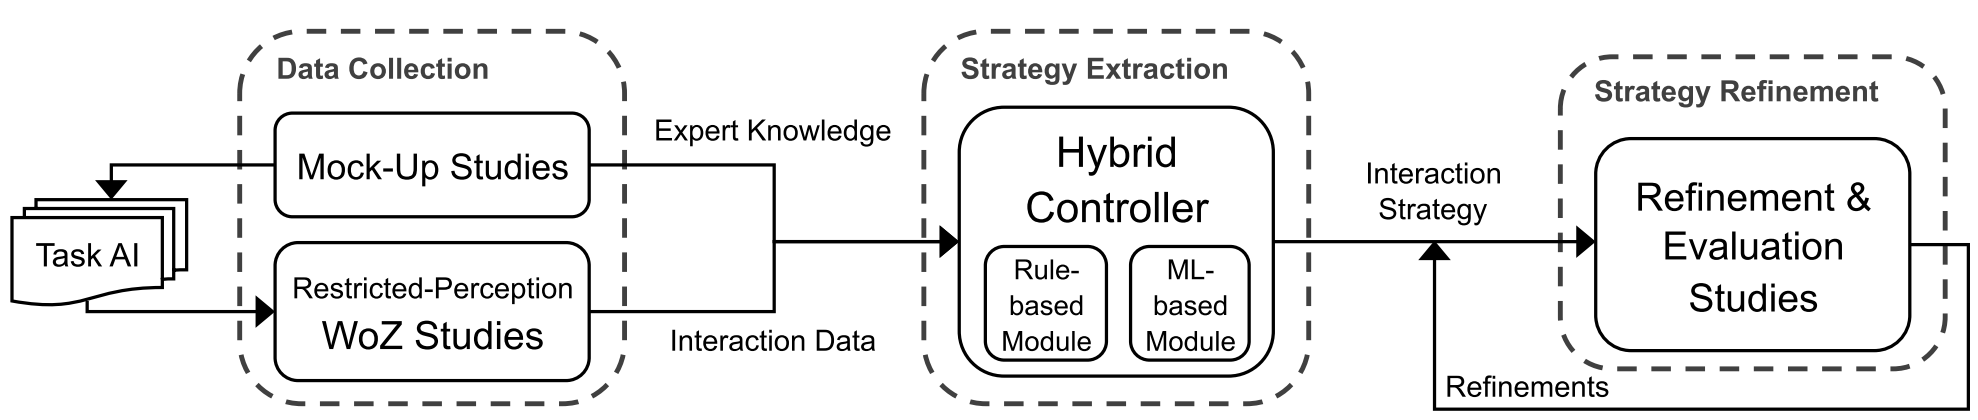
\includegraphics[width=\textwidth]{images/RestrictedPerception_DesignProcess.png}
	\caption{Different stages of the methodology for discovering interaction strategies from restricted-perception \ac{WoZ} studies. From~\cite{Sequeira2016}.}
	\label{fig:RestrictedPerception_DesignProcess}
\end{figure}

%%%%%%%%%%%%%%%%%%%%%%%%%%%%%%%%%%%%%%%%%%%%%%%%%%%%%%%%%%%%%%%%%%%%%%%%%%%%%%%%%
%%%%%%%%%%%%%%%%%%%%%%%%%%%%%%%%%%%%%%%%%%%%%%%%%%%%%%%%%%%%%%%%%%%%%%%%%%%%%%%%%
%%%%%%%%%%%%%%%%%%%%%%%%%%%%%%%%%%%%%%%%%%%%%%%%%%%%%%%%%%%%%%%%%%%%%%%%%%%%%%%%%

\paragraph{\textbf{Evaluation}}

The proposed methodology was tested using a autonomous humanoid tutor capable of learning with young learners in a multiplayer turn-based collaborative video game for building sustainable cities~\cite{Ribeiro2014}. The authors compare the fully-autonomous hybrid controller and a standard unrestricted \ac{WoZ} robot regarding empathy using \ac{IRI}~\cite{Davis1980}, anthropomorphism, animacy, likeability, perceived intelligence and perceived safety of robots using Godspeed series~\cite{Bartneck2009}, and engagement using task-related questionnaires.

%%%%%%%%%%%%%%%%%%%%%%%%%%%%%%%%%%%%%%%%%%%%%%%%%%%%%%%%%%%%%%%%%%%%%%%%%%%%%%%%%
%%%%%%%%%%%%%%%%%%%%%%%%%%%%%%%%%%%%%%%%%%%%%%%%%%%%%%%%%%%%%%%%%%%%%%%%%%%%%%%%%
%%%%%%%%%%%%%%%%%%%%%%%%%%%%%%%%%%%%%%%%%%%%%%%%%%%%%%%%%%%%%%%%%%%%%%%%%%%%%%%%%

\paragraph{\textbf{Discussion}} 

The results showed that empathy was perceived similarly between all conditions but the unrestricted \ac{WoZ} interaction strategies were preferred. The perceived intelligence and security were slightly higher in the restrictive \ac{WoZ}, and the restricted-perception \ac{WoZ} based robots were able to engage very naturally in socially-aware interactions.

This approach requires more preparation than the unrestricted \ac{WoZ} and, as the author suggests, even by using restrictive \ac{WoZ}, it is difficult to isolate the human expert's implicit knowledge regarding the environment.

To conclude, the most important aspects that may contribute to the proposed solution are:
\begin{itemize}
	\item Use of mockup-studies to gain preliminary insight of common patterns in human behaviour;
	\item Restricting the wizard's perceptions to the same extent as the agent;
	\item Use of an iterative approach to further refine the model in each iteration;
	%\item Usage of lazy learning to reduce overfitting issues;
	\item Hybrid controller with rule-based and \ac{ML}-based modules for simple and more complex perceptual states, respectively;
	\item Usage of thinking aloud technique to gain further insight on the users~\cite{Nielsen1992}.
\end{itemize}
% https://www.lightbluetouchpaper.org/2007/03/14/how-not-to-write-an-abstract/
% http://web.ece.ucdavis.edu/~jowens/biberrors.html

\subsection{Overall Discussion}
\label{subsec:RelWorkDiscussion}

Developing a computational models capable of managing rapport similarly to humans is not an easy feat. Researchers had to focus their research on different aspects of rapport and assess their overall contribution. Table~\ref{fig:comparison:rapportSystems} and Table~\ref{fig:comparison:vh:systems}, respectively, compares the systems regarding how they learn social behaviours, and the used rapport management strategies.

\addtolength{\tabcolsep}{1pt}
\begin{table}
	\centering
	\begin{tabular}{lccccccccccc}
		& \textbf{Type}
		& \textbf{Agent} 
	  	& \rot[70]{\textbf{Gaze}}
	  	& \rot[70]{\textbf{Backchannel}} 
	  	& \rot[70]{\textbf{Small-Talk}} 
	  	& \rot[70]{\textbf{Facial Expressions}}
	  	& \rot[70]{\textbf{Gestures}} 
	  	& \rot[70]{\textbf{Mirroring}} 
	  	& \rot[70]{\textbf{Smile}}
	  	& \rot[70]{\textbf{Turn Taking}}
	  	& \rot[70]{\textbf{Praise}}
	  	\\
	  	\midrule
	  	%%%%%%%%%%%%%%%%%%%%%%%%%%%%%%%%%%%%%%%%%%%%%%%%%%%%%%%%%%%%%%
	  	Mutlu et al.~\cite{Mutlu2006} & Rule-based & Robotic & \cmark & \xmark & \xmark & \xmark & \xmark & \xmark & \xmark & \xmark & \xmark\\
	  	%%%%%%%%%%%%%%%%%%%%%%%%%%%%%%%%%%%%%%%%%%%%%%%%%%%%%%%%%%%%%%
	  	Stanton et al.~\cite{Stanton2014} & Rule-based & Robotic & \cmark & \xmark & \xmark & \xmark & \xmark & \xmark & \xmark & \xmark & \xmark\\
	  	%%%%%%%%%%%%%%%%%%%%%%%%%%%%%%%%%%%%%%%%%%%%%%%%%%%%%%%%%%%%%%
	  	Andrist et al.~\cite{Andrist2015} & Rule-based  & Robotic & \cmark & \xmark & \xmark & \xmark & \cmark & \xmark & \xmark & \xmark & \cmark\\
	  	%%%%%%%%%%%%%%%%%%%%%%%%%%%%%%%%%%%%%%%%%%%%%%%%%%%%%%%%%%%%%%
	  	Mohammad et al.~\cite{Mohammad2010} & \ac{ML}-based  & Robotic & \textbf{?} & \cmark & \xmark & \xmark & \xmark & \xmark & \xmark & \xmark & \xmark \\ 
	  	%%%%%%%%%%%%%%%%%%%%%%%%%%%%%%%%%%%%%%%%%%%%%%%%%%%%%%%%%%%%%%
	  	Huang et al.~\cite{Buschmeier2011} & \ac{ML}-based & Virtual & \xmark & \cmark & \cmark & \cmark & \cmark & \cmark & \cmark & \xmark & \xmark\\
	  	%%%%%%%%%%%%%%%%%%%%%%%%%%%%%%%%%%%%%%%%%%%%%%%%%%%%%%%%%%%%%%
	  	Kok et al.~\cite{Kok2012} & \ac{ML}-based & Virtual &  \xmark & \cmark & \xmark & \xmark & \cmark & \xmark & \xmark & \xmark & \xmark\\
	  	%%%%%%%%%%%%%%%%%%%%%%%%%%%%%%%%%%%%%%%%%%%%%%%%%%%%%%%%%%%%%%
	  	Schröder et al.~\cite{Schroder2012} & \ac{ML}-based & Virtual & \xmark & \cmark & \xmark & \cmark & \cmark & \xmark & \xmark & \cmark & \xmark\\
  		\bottomrule
	\end{tabular}
	\caption{Brief comparison regarding how different virtual agents manage strategies. The systems presented here appear in the same order as in the main body of the text.  \protect\cmark, \protect\xmark \, and \textbf{?}, represents whether the specified strategy is applied, not applied or unclear, respectively.}
	\label{fig:comparison:rapportSystems}
	
\end{table}
\addtolength{\tabcolsep}{-1pt}

Current literature suggests continuing the research on learning social behaviours from \ac{WoZ}~\cite{Sequeira2016, Knox2014, Papangelis2014} studies and use primarily \ac{RL}~\cite{Thomaz2006, Kok2012, Zhao2014, Papangelis2014} classifiers (Section~\ref{subsec:ReinforcementLearning}). This class of algorithms are applicable in rapport as there are sequences of states that will help the agent to know when and how backchannels should be produced in order to build rapport (the reward function). In addition, authors suggest developing solutions capable of adapting current course of actions to the current context of the interaction to improve the quality of virtual agents during interactions~\cite{Kopp2007, Zwiers2011, Reidsma2011, Visser2014}.

\begin{table}[]
	\centering
	\begin{tabular}{|l|c|c|}
		\hline
		\textbf{System}              	& \textbf{Training Source} 	& \textbf{Iterative} \\ \hline
		%%%%%%%%%%%%%%%%%%%%%%%%%%%%%%%%%%%%%%%%%%%%%%%%%%%%%%%%%%%%%%%%%%%%%%%%%%%%%%%%%%%%%%%%%%%%%%%%%
		Mohammad et al.~\cite{Mohammad2010} & Direct Samples (Unsupervised) & Yes \\ \hline
		%%%%%%%%%%%%%%%%%%%%%%%%%%%%%%%%%%%%%%%%%%%%%%%%%%%%%%%%%%%%%%%%%%%%%%%%%%%%%%%%%%%%%%%%%%%%%%%%%
		Virtual Rapport 2.0~\cite{Buschmeier2011} 			& Corpus			& No \\ \hline
		%%%%%%%%%%%%%%%%%%%%%%%%%%%%%%%%%%%%%%%%%%%%%%%%%%%%%%%%%%%%%%%%%%%%%%%%%%%%%%%%%%%%%%%%%%%%%%%%%
		\acf{IPL}~\cite{Kok2012}          				& Corpus \& Subjective evaluation			& Yes \\ \hline
		%%%%%%%%%%%%%%%%%%%%%%%%%%%%%%%%%%%%%%%%%%%%%%%%%%%%%%%%%%%%%%%%%%%%%%%%%%%%%%%%%%%%%%%%%%%%%%%%%
		\acf{SAL}~\cite{Schroder2012} & Corpus \& \ac{WoZ}		& Yes \\ \hline
		%%%%%%%%%%%%%%%%%%%%%%%%%%%%%%%%%%%%%%%%%%%%%%%%%%%%%%%%%%%%%%%%%%%%%%%%%%%%%%%%%%%%%%%%%%%%%%%%%
		Restricted Perception~\ac{WoZ}~\cite{Sequeira2016}  & \ac{WoZ}		& Yes \\ \hline
		
	\end{tabular}
	\caption{Brief comparison of methodologies to learn human social behaviours.}
	\label{fig:comparison:vh:systems}
\end{table}

Most of all, the communication goals of interactions must be considered when developing rapport agents. The context in which the communication partners will interact, the inherent limitations of the virtual agents' perceptions and actions and, most importantly, what kind of emotions and actions we want to elicit from the conversational partner are crucial for the development of such agents. For example, in tutoring applications, mutual gaze plays an important role for increased learning performance \cite{OTTESON1980, SHERWOOD1987, Fry1975}, and in negotiation scenarios not reciprocating negative self-disclosure has ben shown to destroy rapport\cite{Bronstein2012}.

